\section{Experiments}

\subsection{Experimental Settings}
\paragraph{Datasets}
%Describe the two datasets.
We evaluate our approach on two datasets, including one English datasets and one Chinese dataset.

The English dataset, DBpedia dataset, is the one generated by \cite{chen2014encoding}, by mapping the triples in DBpedia \cite{bizer2009dbpedia} to the sentences in New York Time corpus. It has 51 different relations, includes about 50,000 entity tuples, 134,000 sentences for training and 30,000 entity tuples, 53,000 sentences for testing.

The Chinese dataset, HudongBaiKe dataset, is also generated by \cite{chen2014encoding}, they derive knowledge facts and construct a Chinese KB from the Infoboxes of HudongBaiKe, one of the largest Chinese online encyclopedias. They collect four national economic newspapers in 2009 as their corpus. 28 different relations are mapped to the corpus and this results in 60,000 entity tuples, 120,000 sentences for training and 40,000 tuples, 83,000 sentences for testing.

\paragraph{Hyperparameters}
%Describe the hyper parameters.
We use a grid search to determine the optimal parameters. For the Base Model(CNN), the CNN window size is 3, the Sentence embedding size is 256, position dimension is 5, batch size is 50, and the word embedding size is 50 for DBpedia dataset, 300 for Chinese dataset.

\iffalse
\begin{table}[!t]  
	\centering  
	\scriptsize  
	\caption{Parameter settings}  
	\begin{tabular}{ll}  
		\\[-2mm]  
		\hline  
		\hline\\[-2mm]
		\vspace{1mm} 
		CNN Window size      &   \tabincell{l}{3}\\  
		\vspace{1mm}  
		Sentence embedding size       &   \tabincell{l}{256}\\  
		\vspace{1mm}  
		English Word dimension  &   \tabincell{l}{50}\\  
		\vspace{1mm}  
		Chinese Word dimension  &   \tabincell{l}{300}\\  
		\vspace{1mm}  
		Position dimension       &   \tabincell{l}{5}\\  
		\vspace{1mm}  
		Batch size        &   \tabincell{l}{50}\\
		\vspace{1mm}  
		Learning rate       &   \tabincell{l}{0.001}\\
		\vspace{1mm}  
		Semantic loss rate        &   \tabincell{l}{0.001}\\
		\hline  
		\hline  
	\end{tabular} 
	
	\label{tab:notations}  
\end{table} 
\fi

\subsection{Experimental Results}
%We evaluate PR-curve (briefly introduce the PR-curve) for SL, base model, ILP, simplified SL.
We use the Precision-Recall curve as the evaluation criterion in our experiments. To prove our approach make sense, we compare our results with baseline CNN model \cite{lin2016neural} and ILP method \cite{chen2014encoding}. The results on DBpedia Dataset and Chinese Dataset are showed in Figure 1 and Figure 2.
\begin{figure}[htbp]
	\centering
	\begin{minipage}[t]{0.48\textwidth}
		\centering
		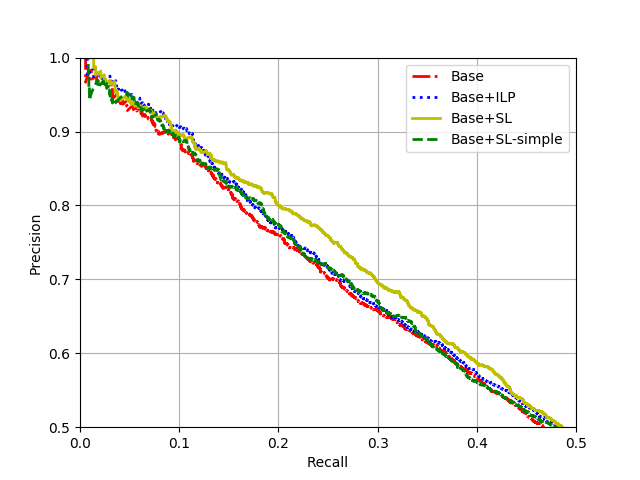
\includegraphics[width=8cm]{./result-figure/DBpedia-CNN-result.png}
		\caption{The DBpedia Dataset}
	\end{minipage}
	\begin{minipage}[t]{0.48\textwidth}
		\centering
		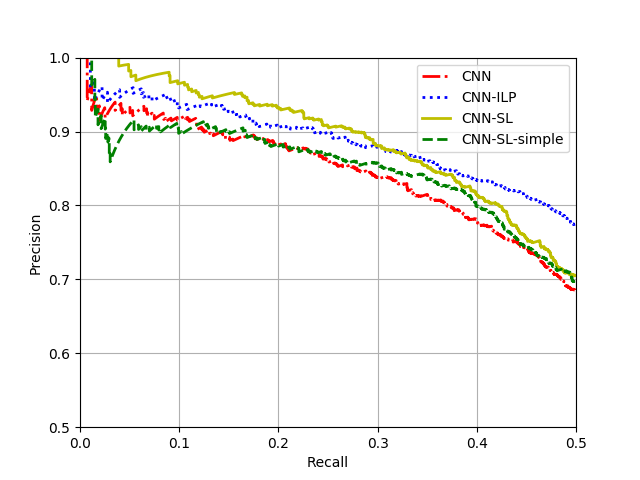
\includegraphics[width=8cm]{./result-figure/Chinese-CNN-result.png}
		\caption{The Chinese Dataset}
	\end{minipage}
\end{figure}

\paragraph{Compare with Base Model}
%Compare the semantic loss method and the base model (clear improvement).
Figure 1 shows that compared with the baseline, our framework performs consistently better in the DBpedia dataset and Chinese dataset. In order to father demonstrate the semantic loss term helps to encode the constraints into relation extraction model, we count the tuple pairs that violates relation constraints introduced in Sec.~\ref{sec:constraints}, the results is show in Table ~\ref{table:violate-count}.

\begin{table}
	\centering  
	\scriptsize  
	\caption{violate count}  
	\begin{tabular}{|c|c|c|c|c|}  
		\hline  
		 &Model&Type Violates&Cardinality Violates&Total\\  
		\hline 
		\multirow{2}*{DBpedia} & CNN & - & - & -\\
		~ & CNN-SL & - & - & -\\
		\hline 
		\multirow{2}*{Chinese} & CNN & - & - & -\\
		~ & CNN-SL & - & - & -\\ 
		\hline   
	\end{tabular} 
	
	\label{table:violate-count}  
\end{table}

\iffalse
\begin{figure}
	\centering
	\includegraphics[width=.4\textwidth]{./result-figure/CNN0-1.png}
	\caption{The DBpedia Dataset}
\end{figure}
\fi


\paragraph{Compare with ILP Method}
Compare the semantic loss method and ILP.

NOTE: clw also use cardinality constraints

\paragraph{Compare with Simplified Semantic Loss}
Compare the semantic loss method and the simplified semantic loss.
Both on PR-curve, and on time.




